In order to further optimize the code some profiling is needed to identify the bottleneck and solve them... If possible. \\
\section{Finding CPU hotspots}
The methodology followed is to use \textbf{Intel VTune} on the entire regression. Profiling only the nnls portion of the code did not give reliable results because terminates too fast. Profiling the entire regression instead, gave interesting results; As showed in \ref{img:vtune_eigen_01} and \ref{img:vtune_eigen_02} there are two hotspots in the code. \\
\begin{figure}[ht]
  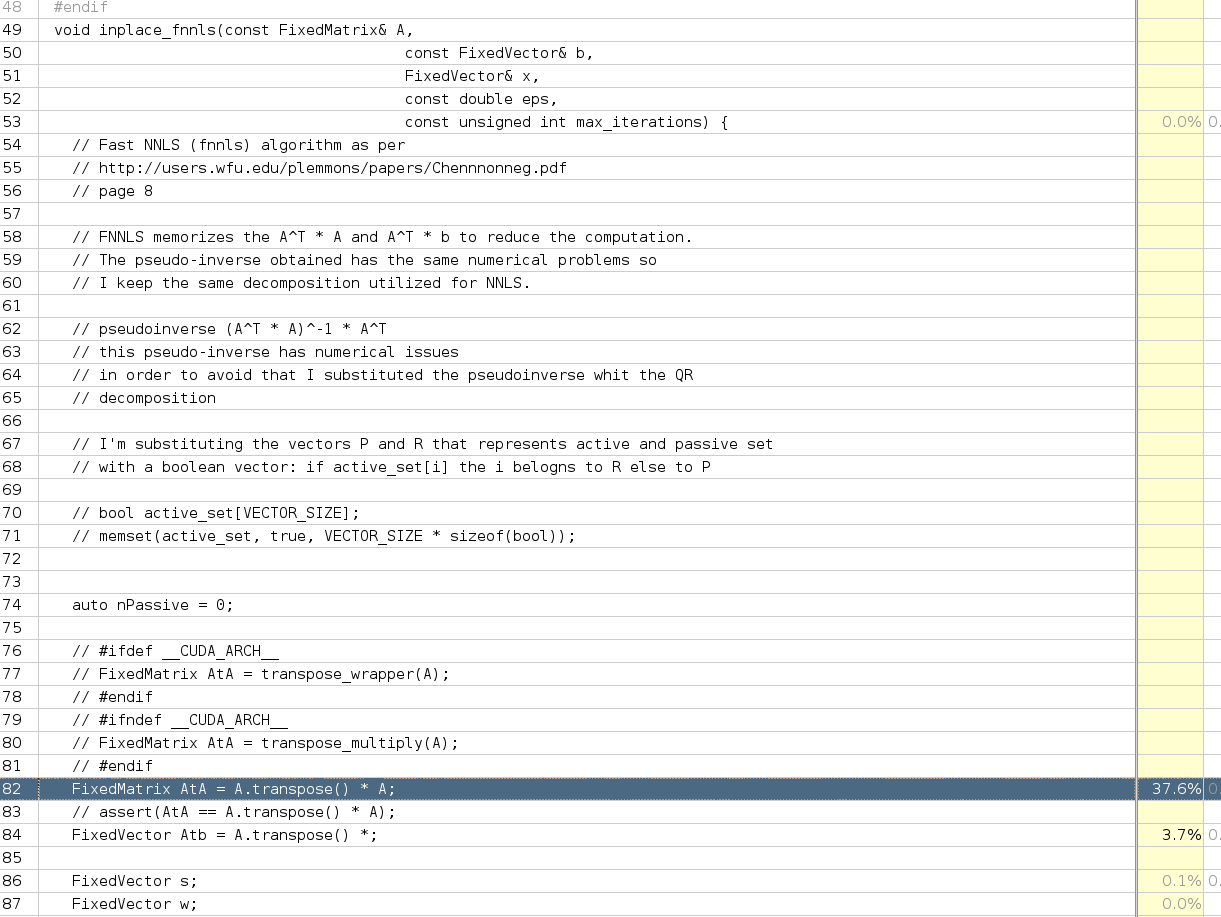
\includegraphics[width=\textwidth]{img/vtune_eigen_01}
  \caption{VTune profiling of multifit\_cpu. 37\% of the total time is spent performing $A^TA$.}
  \label{img:vtune_eigen_01}
\end{figure}
\begin{figure}[ht]
  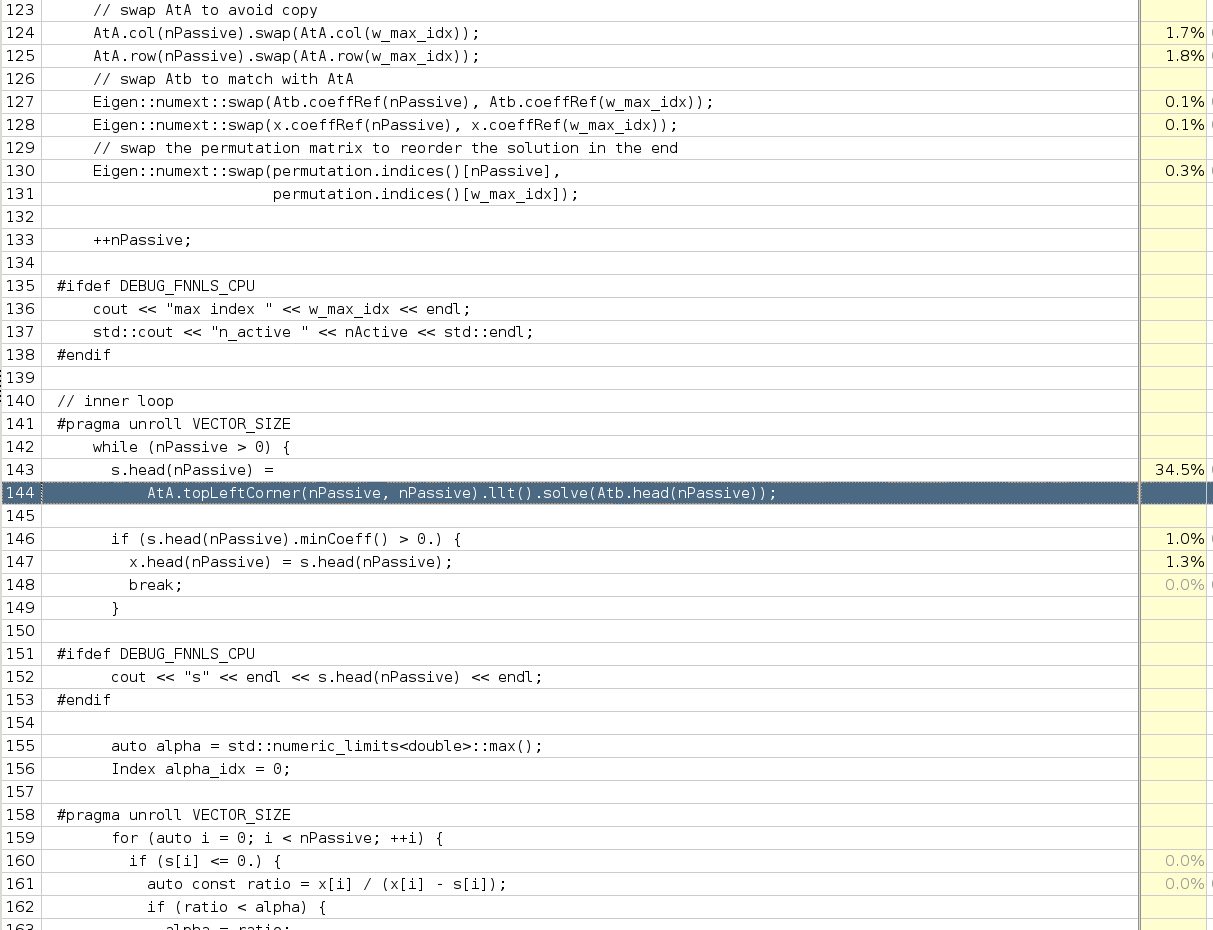
\includegraphics[width=\textwidth]{img/vtune_eigen_02}
  \caption{Second bottleneck found using VTune. 34\% of the time is spent calculating the Cholesky decomposition.}
  \label{img:vtune_eigen_02}
\end{figure}
\subsection{Matrix multiplication}
The first hotspot is the computation of $A^TA$ that requires 37\% of the total execution time. To solve this hotspot it is possible by exploiting the observations:
\begin{itemize}
    \item The matrix $A^TA$ is symmetric so it is enough calculate the one triangular portion and the copy the results back.
    \item The matrix is $10 \times 10$, it fits in L1 cache, thus cache efficiency is more important than algorithmic complexity.
\end{itemize}
\begin{figure}[ht]
  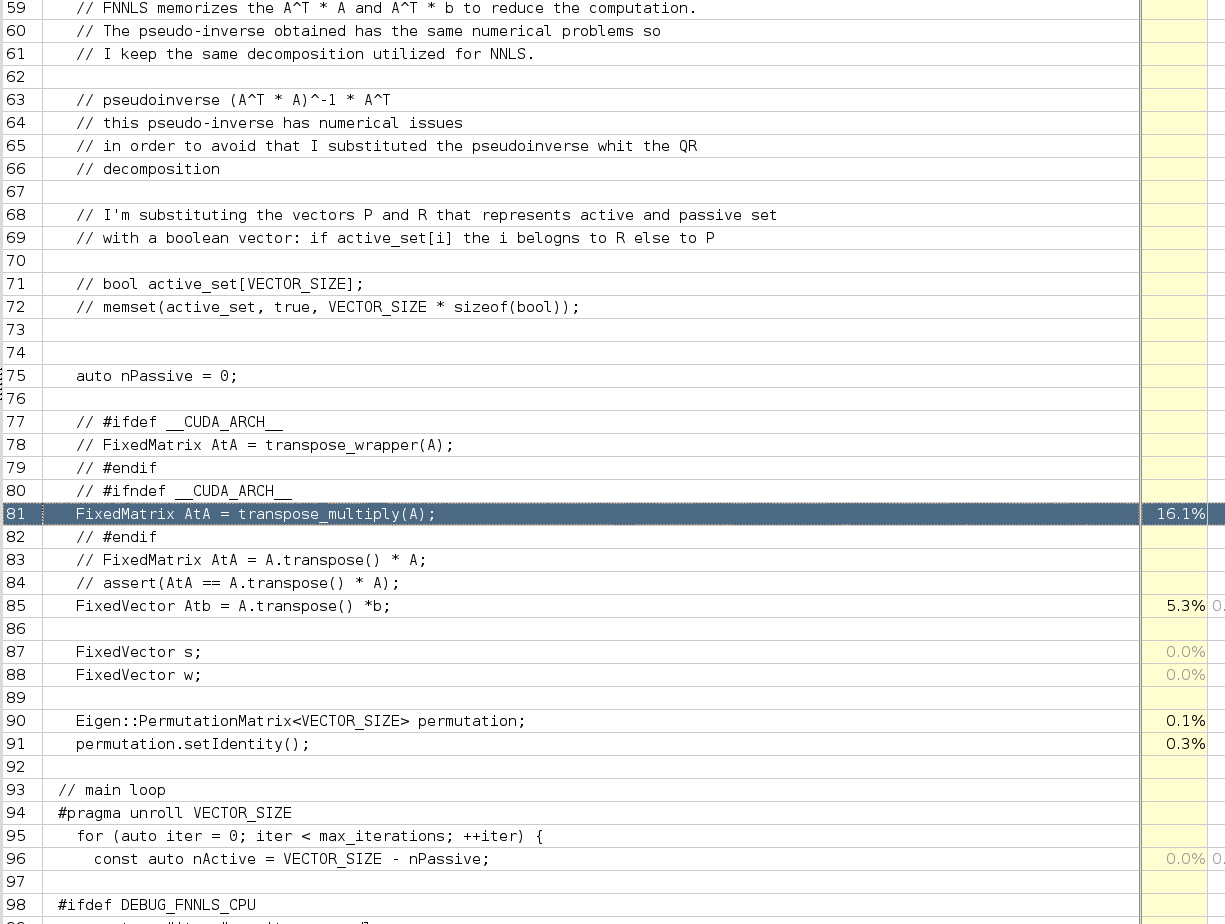
\includegraphics[width=\textwidth]{img/vtune_mine}
  \caption{Cache efficient $10 \times 10$ matrix multiplication. The time needed to perform it is only 16.1\% respect to the 37.6\% spent by eigen implementation.}
  \label{img:vtune_mine}
\end{figure}
Exploiting the hypothesis stated above the implementation illustraded in pseudo-code \ref{alg:transpose_multiply}, specific for this case, has been provided.\\
\begin{algorithm}[h]
  \begin{flushleft}
    \caption{Cache efficient matrix transposition and multiplication. A column major storage order is assumed otherwise the index needs to be reversed.}
    \label{alg:transpose_multiply}
    \textbf{Input:} \\
    \hspace*{\algorithmicindent} \text{\textbf{A} real valued matrix of dimension $m \times n$}\\
    \textbf{Output:} \\
    \hspace*{\algorithmicindent} \text{\textbf{$\bm{A^TA}$} Real valued matrix of size $m \times m$}
  \end{flushleft}
  \begin{algorithmic}[1]
    \Function{transpose\_multiply}{$\protect{A}$}
    \State $m \times m$ matrix $B$
      \For {$i \gets 0$; $i < m$; $++i$}
        \For {$j \gets i$; $j < m$; $++j$} \Comment{$A^TA$ is symmetric, compute half of it}
        \State $B_{ji} \gets 0$
        \For {$k \gets 0$; $k < m$; $++j$}
        \State $B_{ji}+=A_{ik}*A_{jk}$
        \EndFor
        \State $B_{ij} \gets B_{ji}$ \Comment{Copy the result on the other half}
        \EndFor
        \EndFor
        \Return{$B$}
        \EndFunction
      \end{algorithmic}
    \end{algorithm}
This code is very simple but, in cache simple things are needed. The goal is to avoid useless computations, cache faults, and bubbles generated by branches. The main idea behind it is given that $A^TA$ is symmetric compute only half of it and copy the values to the other part. Moreover, knowing that the multiplication is not between two random matrices but, between a matrix and his transpose, if the storage order is column major perform a column$\times$column dot product or a row$\times$row one in the other case. Since the storage order is column major there is another minor optimization that can be performed to gain the last drop of performance. This optimization is about the loop order. A careful choice minimizes jumps, for example in this particular case iterate over column generates no jumps neither cache misses, while iterating over rows generate a jump. A loop order of $row \rightarrow column \rightarrow dot\ product$ means that for each row there is one and only one jump. Instead, a loop order like $column \rightarrow row \rightarrow dot\ product$ generates $|columns| \times |rows|$ jumps, which is bad for performance. \\
This optimized version of the matrix multiplication, as showed in \ref{img:vtune_mine} takes only 16.1\% of the total time, while the reference one takes 37.6\% of it, giving a speedup of $2.33$.\\
On the GPU side instead, is it possible to optimize this further by parallelizing this product with a kernel invocation. \\
\subsection{Updating the Cholesky}
The second bottleneck can be solved using the closed formula present in \cite{wiki:Cholesky_decomposition} to update the Cholesky without recomputing it in case of adding/removing one column and one row.\\
Given that nnls updates a components of the solution vector at the time, to reduce the number of iterations performed inside the regression it is possible to directly exploit this information to update the $\Sigma$ matrix. That way the whole regression, that is intrinsically iterative might be executed in fewer iterations.\\

